\documentclass{standalone}
\usepackage{tikz}
\usetikzlibrary{patterns, positioning}
\usepackage[sfdefault]{ClearSans} %% option 'sfdefault' activates Clear Sans as the default text font
\usepackage[T1]{fontenc}

\begin{document}
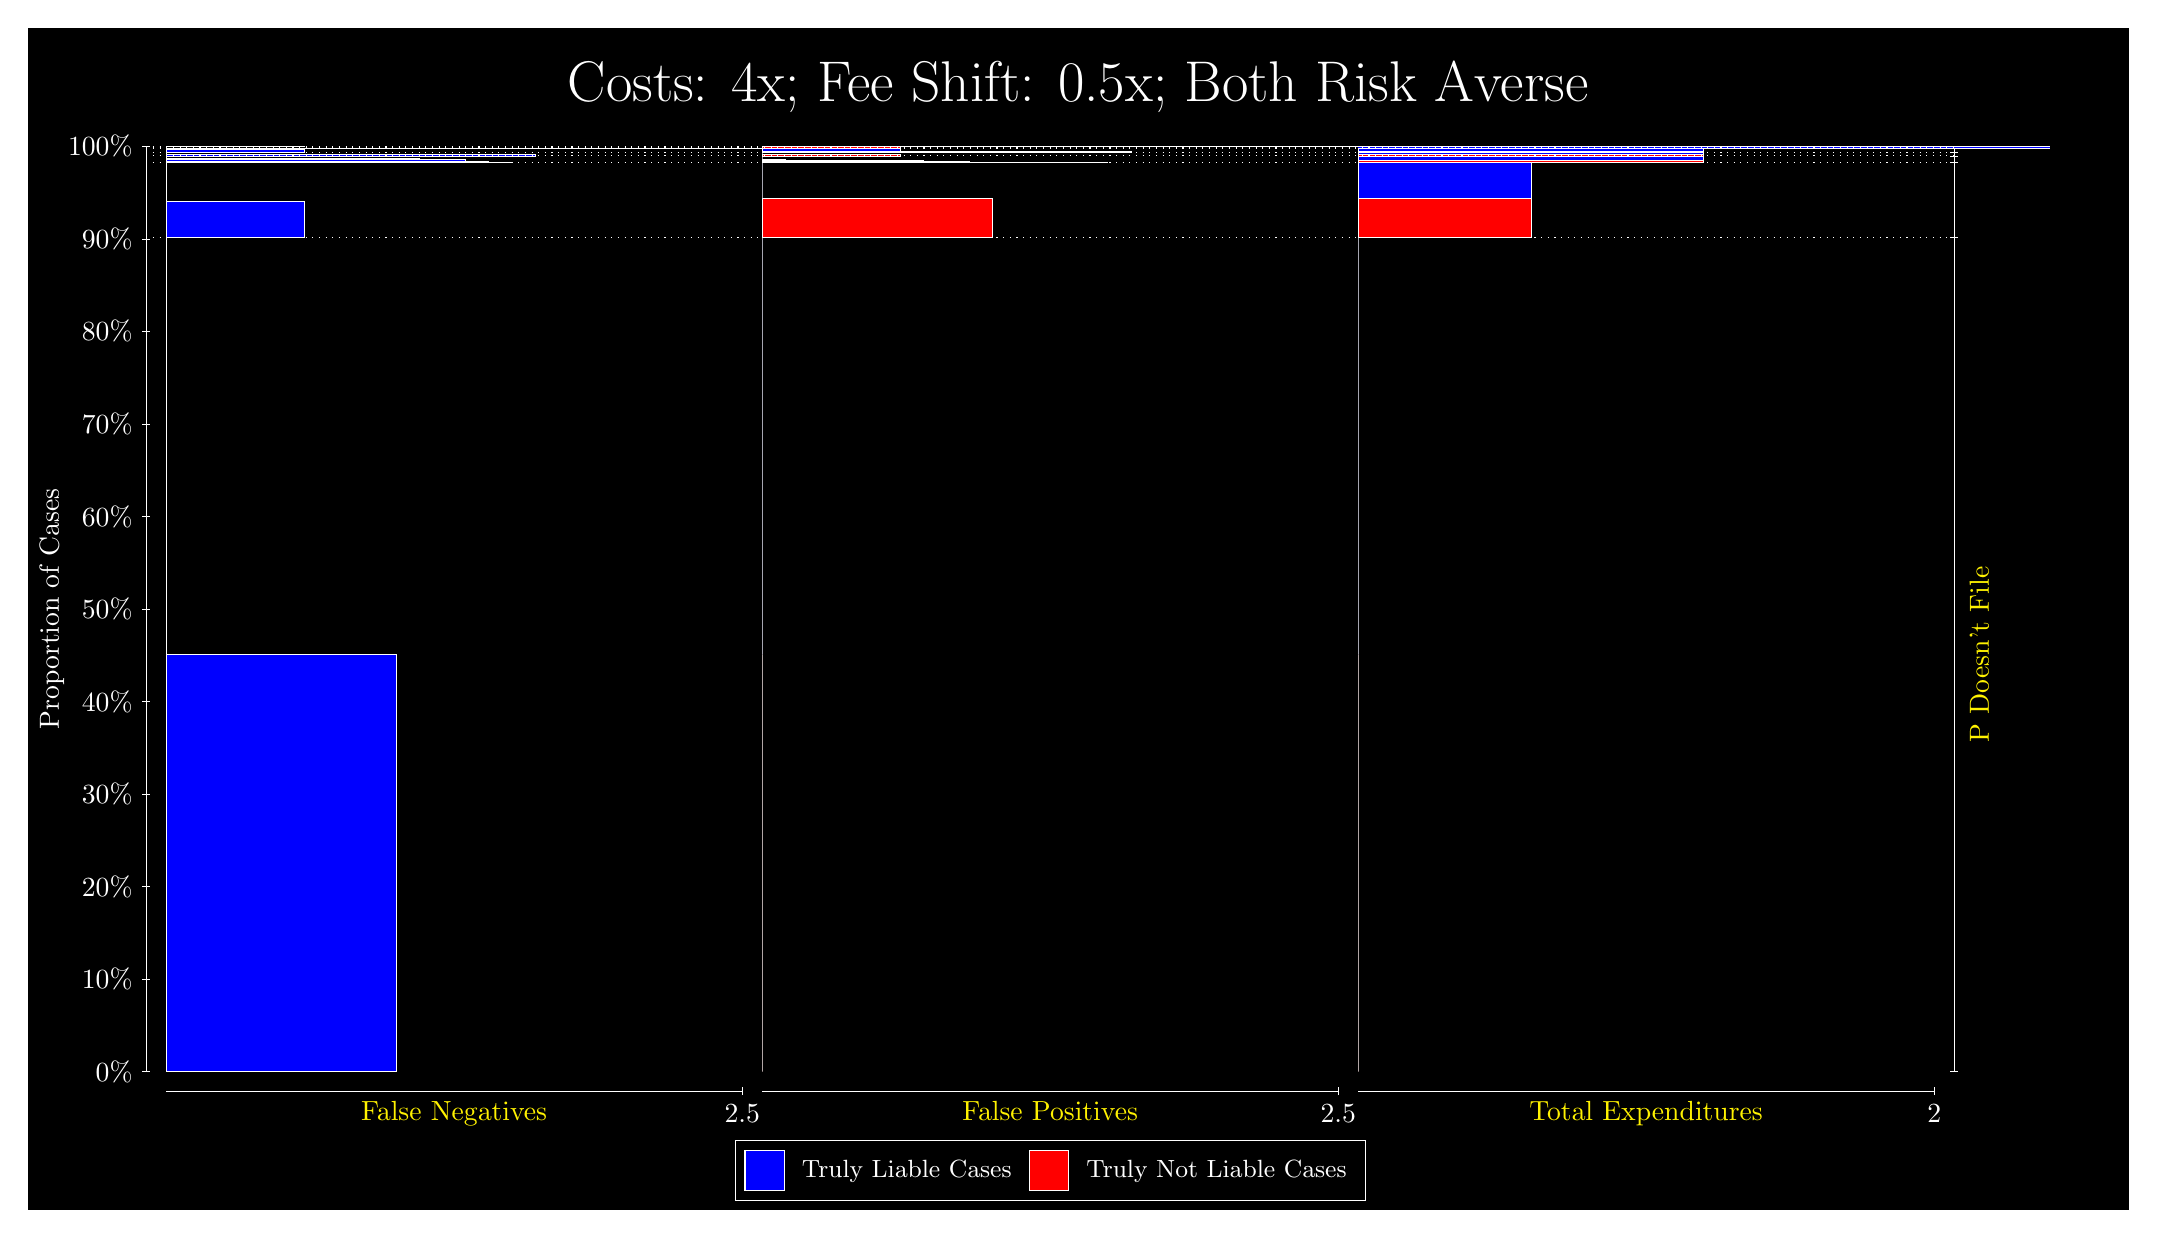
\begin{tikzpicture}
\draw[fill=black] (0,0) rectangle (26.667,15);
\draw[text=white] (0,13.5) rectangle (26.667,15) node[midway] {\huge Costs: 4x; Fee Shift: 0.5x; Both Risk Averse};
\draw[white, very thin] (1.5,1.75) -- (1.5,13.5);
\node[rotate=90, text=white, anchor=center] at (0.3, 7.625) {Proportion of Cases};
\draw[white, very thin] (1.45,1.75) -- (1.55,1.75);
\node[text=white, anchor=east] at (1.45, 1.75) {0\%};
\draw[white, very thin] (1.45,2.925) -- (1.55,2.925);
\node[text=white, anchor=east] at (1.45, 2.925) {10\%};
\draw[white, very thin] (1.45,4.1) -- (1.55,4.1);
\node[text=white, anchor=east] at (1.45, 4.1) {20\%};
\draw[white, very thin] (1.45,5.275) -- (1.55,5.275);
\node[text=white, anchor=east] at (1.45, 5.275) {30\%};
\draw[white, very thin] (1.45,6.45) -- (1.55,6.45);
\node[text=white, anchor=east] at (1.45, 6.45) {40\%};
\draw[white, very thin] (1.45,7.625) -- (1.55,7.625);
\node[text=white, anchor=east] at (1.45, 7.625) {50\%};
\draw[white, very thin] (1.45,8.8) -- (1.55,8.8);
\node[text=white, anchor=east] at (1.45, 8.8) {60\%};
\draw[white, very thin] (1.45,9.975) -- (1.55,9.975);
\node[text=white, anchor=east] at (1.45, 9.975) {70\%};
\draw[white, very thin] (1.45,11.15) -- (1.55,11.15);
\node[text=white, anchor=east] at (1.45, 11.15) {80\%};
\draw[white, very thin] (1.45,12.325) -- (1.55,12.325);
\node[text=white, anchor=east] at (1.45, 12.325) {90\%};
\draw[white, very thin] (1.45,13.5) -- (1.55,13.5);
\node[text=white, anchor=east] at (1.45, 13.5) {100\%};

\draw[white, very thin] (24.457,1.75) -- (24.457,13.5);
\draw[white, very thin] (24.407,1.75) -- (24.507,1.75);
\node[anchor=west] at (24.407, 1.75) {};
\draw[white, very thin] (24.407,12.344) -- (24.507,12.344);
\node[anchor=west] at (24.407, 12.344) {};
\draw[white, very thin] (24.407,13.295) -- (24.507,13.295);
\node[anchor=west] at (24.407, 13.295) {};
\draw[white, very thin] (24.407,13.379) -- (24.507,13.379);
\node[anchor=west] at (24.407, 13.379) {};
\draw[white, very thin] (24.407,13.422) -- (24.507,13.422);
\node[anchor=west] at (24.407, 13.422) {};
\draw[white, very thin] (24.407,13.479) -- (24.507,13.479);
\node[anchor=west] at (24.407, 13.479) {};
\draw[white, very thin] (24.407,13.496) -- (24.507,13.496);
\node[anchor=west] at (24.407, 13.496) {};
\draw[white, very thin] (24.407,13.5) -- (24.507,13.5);
\node[anchor=west] at (24.407, 13.5) {};

\draw[white, very thin, fill=blue] (1.75,1.75) rectangle (4.6775,7.047);
\draw[white, very thin, fill=red] (1.75,7.047) rectangle (1.75,12.344);
\draw[white, very thin, fill=blue] (1.75,12.344) rectangle (3.5065,12.799);
\draw[white, very thin, fill=red] (1.75,12.799) rectangle (1.75,13.295);
\draw[white, very thin, fill=blue] (1.75,13.295) rectangle (6.1413,13.296);
\draw[white, very thin, fill=blue] (1.75,13.296) rectangle (5.8486,13.315);
\draw[white, very thin, fill=blue] (1.75,13.315) rectangle (5.5558,13.338);
\draw[white, very thin, fill=blue] (1.75,13.338) rectangle (5.2631,13.341);
\draw[white, very thin, fill=blue] (1.75,13.341) rectangle (4.9703,13.344);
\draw[white, very thin, fill=blue] (1.75,13.344) rectangle (4.6775,13.347);
\draw[white, very thin, fill=blue] (1.75,13.347) rectangle (4.3848,13.349);
\draw[white, very thin, fill=blue] (1.75,13.349) rectangle (4.092,13.35);
\draw[white, very thin, fill=blue] (1.75,13.35) rectangle (3.7993,13.351);
\draw[white, very thin, fill=red] (1.75,13.351) rectangle (1.75,13.379);
\draw[white, very thin, fill=blue] (1.75,13.379) rectangle (6.4341,13.398);
\draw[white, very thin, fill=red] (1.75,13.398) rectangle (1.75,13.422);
\draw[white, very thin, fill=blue] (1.75,13.422) rectangle (3.5065,13.467);
\draw[white, very thin, fill=red] (1.75,13.467) rectangle (1.75,13.479);
\draw[white, very thin, fill=blue] (1.75,13.479) rectangle (9.9471,13.481);
\draw[white, very thin, fill=red] (1.75,13.481) rectangle (1.75,13.496);
\draw[white, very thin, fill=blue] (1.75,13.496) rectangle (3.5065,13.498);
\draw[white, very thin, fill=red] (1.75,13.498) rectangle (1.75,13.5);
\draw[white, very thin, fill=red] (9.3189,1.75) rectangle (9.3189,7.0471);
\draw[white, very thin, fill=blue] (9.3189,7.0471) rectangle (9.3189,12.344);
\draw[white, very thin, fill=red] (9.3189,12.344) rectangle (12.246,12.84);
\draw[white, very thin, fill=blue] (9.3189,12.84) rectangle (9.3189,13.295);
\draw[white, very thin, fill=red] (9.3189,13.295) rectangle (13.71,13.295);
\draw[white, very thin, fill=red] (9.3189,13.295) rectangle (13.417,13.296);
\draw[white, very thin, fill=red] (9.3189,13.296) rectangle (13.125,13.297);
\draw[white, very thin, fill=red] (9.3189,13.297) rectangle (12.832,13.298);
\draw[white, very thin, fill=red] (9.3189,13.298) rectangle (12.539,13.3);
\draw[white, very thin, fill=red] (9.3189,13.3) rectangle (12.246,13.301);
\draw[white, very thin, fill=red] (9.3189,13.301) rectangle (11.954,13.309);
\draw[white, very thin, fill=red] (9.3189,13.309) rectangle (11.661,13.315);
\draw[white, very thin, fill=red] (9.3189,13.315) rectangle (11.368,13.323);
\draw[white, very thin, fill=blue] (9.3189,13.323) rectangle (10.783,13.324);
\draw[white, very thin, fill=blue] (9.3189,13.324) rectangle (10.49,13.325);
\draw[white, very thin, fill=blue] (9.3189,13.325) rectangle (10.197,13.327);
\draw[white, very thin, fill=blue] (9.3189,13.327) rectangle (9.9044,13.329);
\draw[white, very thin, fill=blue] (9.3189,13.329) rectangle (9.6116,13.333);
\draw[white, very thin, fill=blue] (9.3189,13.333) rectangle (9.3189,13.379);
\draw[white, very thin, fill=red] (9.3189,13.379) rectangle (11.075,13.403);
\draw[white, very thin, fill=blue] (9.3189,13.403) rectangle (9.3189,13.422);
\draw[white, very thin, fill=red] (9.3189,13.422) rectangle (14.003,13.434);
\draw[white, very thin, fill=blue] (9.3189,13.434) rectangle (11.075,13.479);
\draw[white, very thin, fill=red] (9.3189,13.479) rectangle (11.075,13.495);
\draw[white, very thin, fill=blue] (9.3189,13.495) rectangle (9.3189,13.496);
\draw[white, very thin, fill=red] (9.3189,13.496) rectangle (17.516,13.498);
\draw[white, very thin, fill=blue] (9.3189,13.498) rectangle (14.588,13.5);
\draw[white, very thin, fill=red] (16.888,1.75) rectangle (16.888,7.0471);
\draw[white, very thin, fill=blue] (16.888,7.0471) rectangle (16.888,12.344);
\draw[white, very thin, fill=red] (16.888,12.344) rectangle (19.083,12.84);
\draw[white, very thin, fill=blue] (16.888,12.84) rectangle (19.083,13.295);
\draw[white, very thin, fill=red] (16.888,13.295) rectangle (21.279,13.296);
\draw[white, very thin, fill=blue] (16.888,13.296) rectangle (21.279,13.3);
\draw[white, very thin, fill=red] (16.888,13.3) rectangle (21.279,13.324);
\draw[white, very thin, fill=blue] (16.888,13.324) rectangle (21.279,13.374);
\draw[white, very thin, fill=red] (16.888,13.374) rectangle (21.279,13.376);
\draw[white, very thin, fill=blue] (16.888,13.376) rectangle (21.279,13.379);
\draw[white, very thin, fill=red] (16.888,13.379) rectangle (21.279,13.403);
\draw[white, very thin, fill=blue] (16.888,13.403) rectangle (21.279,13.422);
\draw[white, very thin, fill=red] (16.888,13.422) rectangle (21.279,13.434);
\draw[white, very thin, fill=blue] (16.888,13.434) rectangle (21.279,13.479);
\draw[white, very thin, fill=red] (16.888,13.479) rectangle (25.67,13.495);
\draw[white, very thin, fill=blue] (16.888,13.495) rectangle (25.67,13.496);
\draw[white, very thin, fill=red] (16.888,13.496) rectangle (25.67,13.498);
\draw[white, very thin, fill=blue] (16.888,13.498) rectangle (25.67,13.5);
\draw[white, dotted] (1.5,12.344) -- (24.457,12.344);
\draw[white, dotted] (1.5,13.295) -- (24.457,13.295);
\draw[white, dotted] (1.5,13.379) -- (24.457,13.379);
\draw[white, dotted] (1.5,13.422) -- (24.457,13.422);
\draw[white, dotted] (1.5,13.479) -- (24.457,13.479);
\draw[white, dotted] (1.5,13.496) -- (24.457,13.496);
\draw[white, very thin] (1.75,1.5) -- (9.0689,1.5);
\node[text=yellow, anchor=north] at (5.4094, 1.5) {False Negatives};
\draw[white, very thin] (9.0689,1.45) -- (9.0689,1.55);
\node[text=white, anchor=north] at (9.0689, 1.45) {2.5};

\draw[white, very thin] (9.3189,1.5) -- (16.638,1.5);
\node[text=yellow, anchor=north] at (12.978, 1.5) {False Positives};
\draw[white, very thin] (16.638,1.45) -- (16.638,1.55);
\node[text=white, anchor=north] at (16.638, 1.45) {2.5};

\draw[white, very thin] (16.888,1.5) -- (24.207,1.5);
\node[text=yellow, anchor=north] at (20.547, 1.5) {Total Expenditures};
\draw[white, very thin] (24.207,1.45) -- (24.207,1.55);
\node[text=white, anchor=north] at (24.207, 1.45) {2};

\node[text=yellow, centered, rotate=90] at (24.777, 7.047) {P Doesn't File};







\draw (12.978300999999998,1.5) node[draw=none] (baseCoordinate) {};
\begin{scope}[align=center]
        \matrix[scale=0.5, draw=white, below=0.5cm of baseCoordinate, nodes={draw}, column sep=0.1cm]{
            \node[rectangle, draw, minimum width=0.5cm, minimum height=0.5cm, fill=blue] {}; &
            \node[draw=none, font=\small, text=white] (B) {Truly Liable Cases}; &
            \node[rectangle, draw, minimum width=0.5cm, minimum height=0.5cm, fill=red] {}; &
            \node[draw=none, font=\small, text=white] (B) {Truly Not Liable Cases}; \\
            };
\end{scope}

\end{tikzpicture}
\end{document}